\chapter{Contribution}
In this chapter we propose our data warehouse and visualization system for medical data that aims to manage the uncommon data from the various sources using a conventional common language between the different health actors.




\section{Work Objectives}
The aim of this work is to propose a data warehouse system that organizes data coming from different sources by producing a common language. I NEED SOME BLA BLA HERE.





\section{Literature \& Related works review}
We present in this section architecture for healthcare data warehouses and solutions that attempt to integrate infoVis into medical data and medical structures which could be used by executive managers, doctors, physicians and other health professionals to support the healthcare process.  Medical data existing today in multiple sources with different formats makes it necessary to have certain data integration techniques. A healthcare data warehouse is therefore needed to integrate the different data sources into a central data repository and analyze this data.

\begin{itemize}
  \item \textbf{\textit{A Healthcare Data Warehouse for Cancer Diseases:}} Dr.Osama E.Sheta and Ahmed Nour Eldeen discussed in their paper\cite{shetaBuildingHealthCare2012} the implementation of a healthcare data warehouse for cancer diseases, they proposed  two stages approach for the building cancer data warehouse: 
  \newpage
  \begin{enumerate}
    \item \textit{Business Analysis:} Consist of business process analysis and business requirement analysis (Figure\ref{fig:cancerDiagrame}).
    \begin{figure}[h!]
      \center
      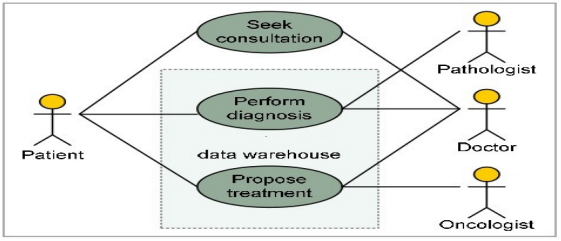
\includegraphics[width=0.75\textwidth]{images/chapter2/cancerDiagrame.PNG}
      \caption{Cancer data warehouse use case diagram.}
      \label{fig:cancerDiagrame}
    \end{figure}
    \item \textit{Architecture Design:} Data is imported from several sources and transformed within a staging area before it is integrated and stored in the production data warehouse for further analysis (Figure\ref{fig:cancersystem}).
     \begin{figure}[h!]
      \center
      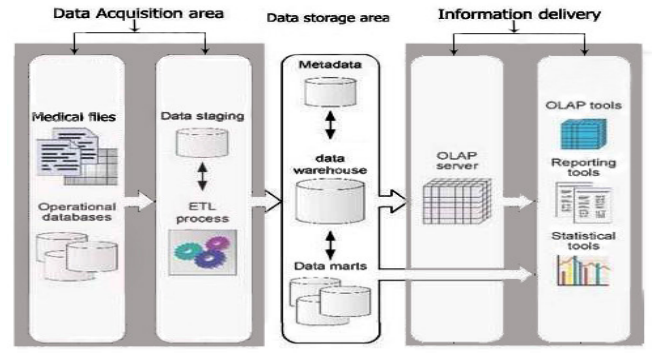
\includegraphics[width=0.75\textwidth]{images/chapter2/cancersystem.PNG}
      \caption{Cancer data warehouse Architecture Taken from the source.}
      \label{fig:cancersystem}
    \end{figure}
    \end{enumerate}
    
    \item \textbf{\textit{Data Warehouse Framework in Pharmaceutical Sector:}} In this paper\cite{abd2019proposed} authors proposed a data warehouse framework to enhance decisions of distribution systems in pharmaceutical companies to decrease the medicine industry cost and increase productivity. The framework can be described in four phases shown in (Figure \ref{fig:pharmacysystem}). Phase one consists of a data preparation phase which has four steps (data collection, building DBs, DWH and data cleaning). Phase two consists of training phase which is applying time series to three types of Neural Networks techniques (levenberg marquardt, Bayesian regularized, and Scaled conjugate gradient).Phase three is testing the performance based on mean square error (MSE). Phase four consists of evaluating the performance of the best prediction model.
    \begin{figure}[h!]
      \center
      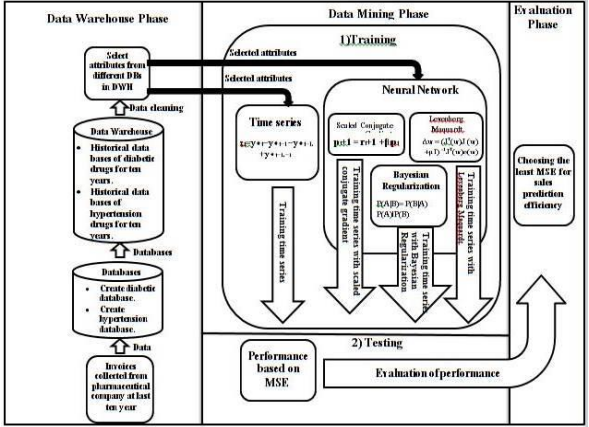
\includegraphics[width=0.75\textwidth]{images/chapter2/pharmacysystem.PNG}
      \caption{The Proposed Framework of Sales Prediction.}
      \label{fig:pharmacysystem}
    \end{figure}
    
    \item \textbf{\textit{Big Bata Warehouse Based On Hadoop Architecture:}} In this paper\cite{sebaa2018medical} entitled “Medical Big Data Warehouse: Architecture and System Design, a Case Study: Improving Healthcare Resources Distribution” authors proposed a system architecture and a conceptual data model for a MBDW (Medical Big Data Warehouse), and then offer a solution to overcome both the growing of fact table size and the lack of primary and foreign keys in the framework Apache Hive required in the conceptual data model. This solution is based on nested partitioning according to the dimension tables keys, then  applying their solution to implement a MBDW to improve medical resources distribution for the health sector in the Bejaia region (in Algeria). 
    \newpage
    The overall architecture is depicted in (Figure \ref{fig:bigdatarelated}). It is a scalable, reliable, and distributed architecture to extract, store, analyze, and visualize healthcare data extracted from various resources HIS (Hospitals Information systems).
    \begin{figure}[h!]
      \center
      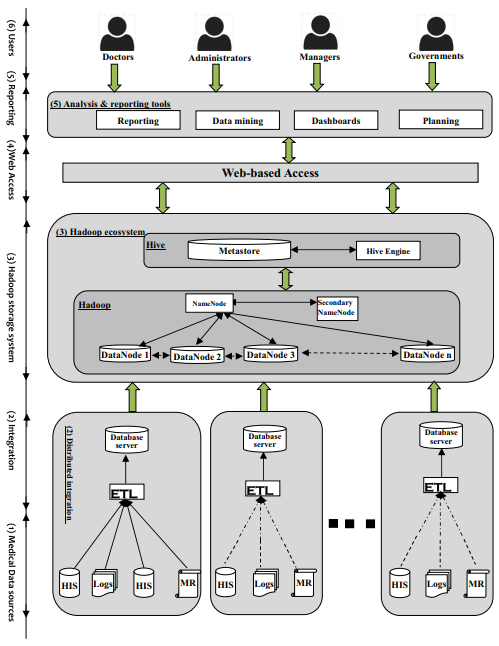
\includegraphics[width=0.50\textwidth]{images/chapter2/relatedworkHadoop.PNG}
      \caption{Hadoop-based system
      architecture of medical big data warehousing.}
      \label{fig:bigdatarelated}
    \end{figure}
\end{itemize}



\section{Diagrams \& Architecture}
